\documentclass[a4paper]{article}

\usepackage{amsmath,amsthm,amssymb}
\usepackage{tikz}
\usetikzlibrary{arrows}
\usetikzlibrary{external}
\tikzexternalize[prefix=figures/]

\tikzset{
every node/.style={circle, draw, inner sep=2pt},
every label/.style={rectangle, draw=none}
}

\begin{document}

%%%%%%%%%%%%%%%%%%%%%%%%%%%%%%%%%%%%%%%%%%%%%%%%%%
\verb|maptograph|

\tikzsetnextfilename{maptograph}
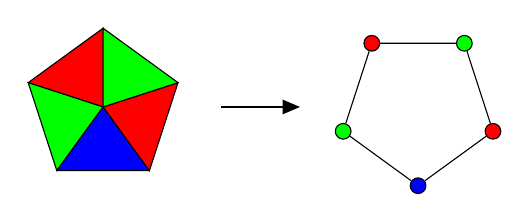
\begin{tikzpicture}
\begin{scope}[xshift=-2cm]
\draw[fill=red] (90:1) -- (0,0) -- (162:1) -- cycle;
\draw[fill=green] (162:1) -- (0,0) -- (234:1) -- cycle;
\draw[fill=blue] (234:1) -- (0,0) -- (306:1) -- cycle;
\draw[fill=red] (306:1) -- (0,0) -- (18:1) -- cycle;
\draw[fill=green] (18:1) -- (0,0) -- (90:1) -- cycle;
\end{scope}

\draw[-triangle 45] (-0.5,0) -- (0.5,0);

\begin{scope}[xshift=2cm]
\node[fill=red] (0) at (126:1) {};
\node[fill=green] (1) at (198:1) {};
\node[fill=blue] (2) at (270:1) {};
\node[fill=red] (3) at (342:1) {};
\node[fill=green] (4) at (54:1) {};
\draw (0) -- (1) -- (2) -- (3) -- (4) -- (0);
\end{scope}
\end{tikzpicture}


\end{document}


%%% compile by pdflatex --shell-escape filename.tex
%%% then run ./pdf2png.sh *.pdf in figures/
